\documentclass[dvipdfmx]{report} % 文章の形式を設定
\usepackage[margin=2.5cm]{geometry} % 書式の空白を設定
\usepackage[utf8]{inputenc} % 文字コードをUTF-8に設定
\usepackage{hyperref} % 目次にリンクを付けるため
\usepackage{lipsum} % ダミーテキスト用
\usepackage{tcolorbox} % 枠を利用するため
\usepackage{amsmath} % 数式の記述を行うため
\usepackage{bm} % ベクトルを太字で表示するため
\usepackage{graphicx} % 画像を表示するため
\usepackage{float} % 画像正しい位置で表示するため
\usepackage{tensor} % テンソルを記載するため
\usepackage{multicol} % 複数段落を作成するため
\usepackage{tikz} % 図を作成するため
\usepackage{amssymb} % 特殊文字を表示するため
\usepackage{enumerate} % リストを作成するため


\title{球対称ブラックホールの像}
\author{Jean-Pierre Luminet}
\date{}

\begin{document}
\maketitle % タイトルの作成

% =================================
% =================================
% =================================
% =================================
% =================================
% bare black hole
% =================================
% =================================
% =================================
% =================================
% =================================
\section{image of bare black hole}
\begin{tcolorbox}[title=シュバルツシルト時空]
	\[
	ds^2 = - \left( 1 - \frac{2M}{r} \right) dt^2 + \left( 1 - \frac{2M}{r} \right)^{-1} dr^2 + r^2 (d\theta^2 + \sin^2 \theta d\phi^2)
	\]
\end{tcolorbox}
この時空を動く光子の軌道を考える。

\subsection{光の測地線方程式}
時空上での光の軌道を表現する式である「光の測地線方程式」を、粒子の場を表す方程式である「クラインゴルドン方程式」から導出する。

\begin{tcolorbox}[title=クラインゴルドン方程式]
	\[
	0 = \left( \frac{1}{c^2}\frac{\partial^2}{\partial t^2} - \nabla^2 + \left( \frac{mc}{\hbar} \right)^2 \right) \phi(\bm{x}, t)
	\]
\end{tcolorbox}
質量のない粒子である光では、項がひとつ減って

\begin{equation*}
\begin{split}
	0 &= \left( \frac{1}{c^2}\frac{\partial^2}{\partial t^2} - \nabla^2 \right)\phi(\bm{x}, t)\\
	&= \square \phi(\bm{x}, t)
\end{split}
\end{equation*}
と書ける。これを一般の時空に拡張すると
\[ 0 = g^{ij} \nabla_i \nabla_j \phi \]
ここで
\[ \phi = Ce^{i\frac{s}{\epsilon}} \] 
と書くと
\begin{equation*}
\begin{split}
	\nabla_j \phi &= \nabla \left( Ce^{\frac{is}{\epsilon}} \right)\\
	&= \left( \nabla_j C \right) e^{\frac{is}{\epsilon}} + \frac{iC}{\epsilon} e^{\frac{is}{\epsilon}} \left( \nabla_j S \right)\\
	\nabla_i \nabla_j \phi &= \nabla_i \left(  \left( \nabla_j C \right) e^{\frac{is}{\epsilon}} + \frac{iC}{\epsilon} e^{\frac{is}{\epsilon}} \left( \nabla_j S \right) \right)\\
	&= \left( \nabla_i \nabla_j C \right) e^{\frac{is}{\epsilon}} + \left( \nabla_i S \right) \left( \nabla_j C \right) \frac{2i}{\epsilon} e^{\frac{is}{\epsilon}} + \left( \nabla_i \nabla_j S \right) \frac{iC}{\epsilon} e^{\frac{is}{\epsilon}} -  \left( \nabla_i S \right) \left( \nabla_j S \right) \frac{1}{\epsilon^2} e^{\frac{2is}{\epsilon}}\\
	g^{ij} \nabla_i \nabla_j \phi &= g^{ij}\left( \nabla_i \nabla_j C \right) e^{\frac{is}{\epsilon}} + g^{ij}\left( \nabla_i S \right) \left( \nabla_j C \right) \frac{2i}{\epsilon} e^{\frac{is}{\epsilon}} + g^{ij}\left( \nabla_i \nabla_j S \right) \frac{iC}{\epsilon} e^{\frac{is}{\epsilon}} -  g^{ij}\left( \nabla_i S \right) \left( \nabla_j S \right) \frac{1}{\epsilon^2} e^{\frac{2is}{\epsilon}}\\
	&= \left( \square C \right) e^{\frac{is}{\epsilon}} + \left( \nabla_i S \right) \left( \nabla^i C \right) \frac{2i}{\epsilon} e^{\frac{is}{\epsilon}} + \left( \square S \right) \frac{iC}{\epsilon} e^{\frac{is}{\epsilon}} -  \left( \nabla_i S \right) \left( \nabla^i S \right) \frac{1}{\epsilon^2} e^{\frac{2is}{\epsilon}}
\end{split}
\end{equation*}
\begin{equation}
\left\{ \,
\begin{aligned}
	O(\epsilon^{-2}) &: \left( \nabla_i S \right) \left( \nabla^i S \right) = 0\\
	O(\epsilon^{-1}) &: 2 \left( \nabla_i S \right) \left( \nabla^i C \right) + C \left( \square S \right) = 0\\
	O(0) &: \square C = 0
\end{aligned}
\right.
\end{equation}
ここで、\[ \left( \nabla_i S \right) \left( \nabla^i S \right) = 0 \]は光の測地線方程式を表している。
\[ \nabla_i S  =  k_i \]とおけば
\begin{equation*}
\begin{split}
	0 &= \left( \nabla_i S \right) \left( \nabla^i S \right)\\
	&= k_i k^i\\
	&= \nabla_j (k_i k^i)\\
	&= \nabla_j (k_i g^{ij} k_l)\\
	&= g^{il} (\nabla_j k_l)k_i + g^{il} (\nabla_j k_i)k_l\\
	&= 2(\nabla_j k_i)k^i\\
	&= 2 g^{lj} (\nabla_j \nabla_i S)k^i\\
	&= 2 (\nabla_i g^{lj}  k_j)k^i\\
	&= 2 (\nabla_i k^l)k^i\\
	&= 2\left( \frac{\partial}{\partial x^i} \left( \frac{dx^l}{d\lambda} \right) + \tensor{\Gamma}{^l_{im}} \left( \frac{dx^m}{d\lambda} \right) \right) \frac{dx^i}{d\lambda}
\end{split}
\end{equation*}
\begin{tcolorbox}[title=光の測地線方程式]
\begin{eqnarray*}
	0 = \left( \frac{d^2 x^l}{d\lambda^2} \right) + \tensor{\Gamma}{^l_{im}} \left( \frac{dx^i}{d\lambda}\frac{dx^m}{d\lambda} \right)
\end{eqnarray*}
\end{tcolorbox}



\noindent
/////////////////////////////////////////////////////////////////////////\\
/////////////////////////////////////////////////////////////////////////

% 方程式
\begin{equation*}
\begin{split}
	\bar{w}_j = \left( \right) \int^{}_{}
\end{split}
\end{equation*}

% ボックス
\begin{tcolorbox}[title=メモ用]
\[ 1 = 1 \]
\end{tcolorbox}

% { 付き方程式
\begin{equation}
\left\{ \,
\begin{aligned}
	1 &= 0\\
	1 &= 0\\
\end{aligned}
\right.
\end{equation}

% 画像
% \begin{figure}[H]
%    \centering
%     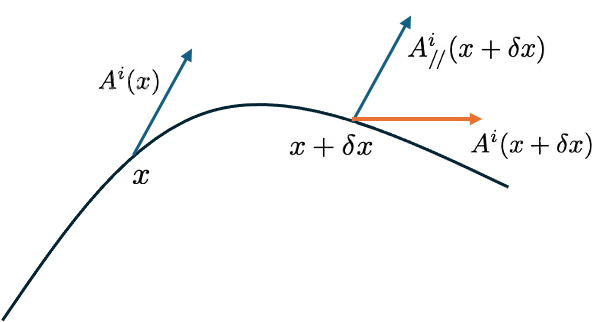
\includegraphics[width=0.5\columnwidth]{./images/0106/01.png}
%     \caption{並行移動}
%     \label{}
% \end{figure}

% リスト
\begin{enumerate}[(1)\,]
\item{}
\end{enumerate}

\end{document}